{\bf BME154L - Spring 2012 - Exam \#2 Solutions}\hfill Name (Net ID):\underline{\hspace*{3.0in}}



\section{[15 points]}

\begin{center}
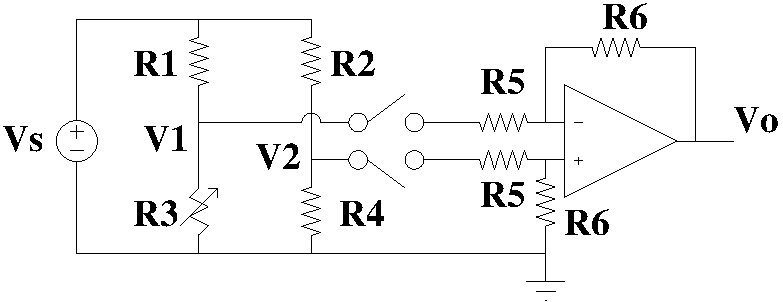
\includegraphics[width=0.65\linewidth]{wheatstone_diff_amp}
\end{center}
 
\begin{enumerate}
    \item Derive expressions for $V_1$ and $V_2$ in terms of $V_s$ and $R_{1-4}$ for this Wheatstone Bridge when the switches are open (as shown).
    \item Derive an expression for $V_2$ in terms of $V_s$ and $R_{1-6}$ for this Wheatstone Bridge when the switches are closed and the differential amplifier is being used to amplify $V_2 - V_1$.  (Note - you do not need to simplify the expression.  Just make sure that it is clear how you set it up!!)
    \item What would be ideal values for $R_5$ and $R_6$ relative to $R_{1-4}$ to prevent corruption of the Wheatstone Bridge output?  If you didn't have control over the values for $R_{1-6}$, then how could you modify the design of this circuit to insure that the output of the Wheatstone Bridge isn't corrupted?
\end{enumerate}

\clearpage

{\bf BME154L - Spring 2012 - Exam \#2 Solutions}\hfill Name (Net ID):\underline{\hspace*{3.0in}}



\clearpage
